\documentclass[11pt]{beamer}

\usetheme{default}
\usecolortheme{seahorse}

\usepackage{amsmath}
\usepackage{amssymb}
\usepackage{graphicx}
\usepackage{hyperref}
\usepackage{listings}
\usepackage{xcolor}
\usepackage{booktabs}

\title{Automated Dynamic Analysis Signature Generation}
\subtitle{Using Large Language Models for Malware Behavior Analysis}
\author{Ikram Benfellah \\ Fadel Fatima Zahra}
\institute{S7 Capstone Project}
\date{March 22, 2026}

\begin{document}

\frame{\titlepage}

\begin{frame}
\frametitle{Table of Contents}
\tableofcontents
\end{frame}

\section{Project Overview}

\begin{frame}
\frametitle{Project Motivation}
\begin{itemize}
  \item Manual malware signature generation is time-consuming and error-prone
  \vspace{0.3cm}
  \item LLMs excel at pattern recognition and semantic understanding
  \vspace{0.3cm}
  \item Goal: Automate CAPEv2 signature generation from sandbox behavioral logs
  \vspace{0.3cm}
  \item Innovation: First LLM integration with CAPEv2 Python signature generation
\end{itemize}
\end{frame}

\begin{frame}
\frametitle{Research Questions}
\begin{enumerate}
  \item What is the quality of LLM-generated signatures (precision/recall/F1)?
  \vspace{0.3cm}
  \item How well do signatures generalize to unseen malware families?
  \vspace{0.3cm}
  \item How accurate is automated MITRE ATT\&CK technique mapping?
\end{enumerate}
\end{frame}

\section{System Architecture}

\begin{frame}
\frametitle{Six-Stage Pipeline}
\begin{enumerate}
  \item \textbf{Data Acquisition}: Load CAPEv2 sandbox reports
  \item \textbf{Feature Extraction}: Extract behavioral features
  \item \textbf{Behavior IR}: Build unified representation
  \item \textbf{LLM Analysis}: Semantic interpretation
  \item \textbf{Signature Generation}: Create Python signatures
  \item \textbf{Evaluation}: Comprehensive assessment
\end{enumerate}

\vspace{0.3cm}
\textbf{Dataset}: 100 malware samples from 10 families (Emotet, Zeus, Trickbot, etc.)
\end{frame}

\section{Methodology}

\begin{frame}
\frametitle{Feature Extraction}
\begin{itemize}
  \item Process operations (creation, injection, termination)
  \item Registry modifications (run keys, startup entries)
  \item File I/O operations (creation, execution, overwrites)
  \item Network activity (DNS, TCP, HTTP/HTTPS, C2)
  \item API call sequences and patterns
\end{itemize}

\vspace{0.3cm}
\textbf{Output}: 50+ behavioral features per sample
\end{frame}

\begin{frame}
\frametitle{Behavior Intermediate Representation}
\begin{itemize}
  \item Normalizes CAPEv2 format into unified JSON structure
  \item Groups behaviors by category
  \item Enables LLM semantic analysis without raw complexity
  \item Includes temporal sequencing information
\end{itemize}
\end{frame}

\begin{frame}
\frametitle{LLM-Based Semantic Analysis}
\begin{enumerate}
  \item Convert behaviors to natural language descriptions
  \item Per-sample LLM analysis with threat level assessment
  \item Family-level pattern aggregation
  \item Cache all results for reproducibility
\end{enumerate}

\vspace{0.3cm}
\textbf{Benefits}:
\begin{itemize}
  \item Semantic understanding of complex behaviors
  \item Automated threat characterization
  \item Reproducible analysis pipeline
\end{itemize}
\end{frame}

\begin{frame}
\frametitle{Signature Generation \& ATT\&CK Mapping}
\begin{enumerate}
  \item Generate CAPEv2 Python signatures from LLM insights
  \item Map behaviors to MITRE ATT\&CK techniques
  \item Validate syntax and test coverage
\end{enumerate}

\vspace{0.3cm}
\textbf{Output}:
\begin{itemize}
  \item 20 CAPEv2 Python signature files
  \item 35+ MITRE techniques identified
  \item Signature-to-behavior mappings
\end{itemize}
\end{frame}

\section{Results}

\begin{frame}
\frametitle{Signature Generation Results}
\begin{itemize}
  \item Total signatures generated: 20 (2 per family)
  \item Signature generation success rate: 100\%
  \item Python syntax validation: 100\% pass
  \item Families covered: 10/10
\end{itemize}

\vspace{0.3cm}
\textbf{Distribution}:
\begin{itemize}
  \item 5 samples per signature
  \item All CAPEv2-compliant format
  \item Production-ready for deployment
\end{itemize}
\end{frame}

\begin{frame}
\frametitle{MITRE ATT\&CK Mapping}
\begin{itemize}
  \item Unique techniques identified: 35+
  \item Top techniques:
    \begin{itemize}
      \item Process Injection (45 occurrences)
      \item Defense Evasion (38 occurrences)
      \item Persistence (35 occurrences)
      \item Command \& Control (28 occurrences)
    \end{itemize}
\end{itemize}

\vspace{0.3cm}
\textbf{Insights}: All 10 families exhibit multiple ATT\&CK techniques (avg. 8.5 per family)
\end{frame}

\begin{frame}
\frametitle{Behavioral Pattern Coverage}
\begin{itemize}
  \item File Dropping: 81\% coverage (412 events)
  \item Persistence (RunKey): 72\% coverage (156 events)
  \item Process Injection: 67\% coverage (284 events)
  \item C2 Communication: 54\% coverage (203 events)
  \item Defense Evasion: 48\% coverage (165 events)
\end{itemize}

\vspace{0.3cm}
\textbf{Key Finding}: File operations most common, critical behaviors average 64\% coverage
\end{frame}

\begin{frame}
\frametitle{Evaluation Metrics}
\begin{itemize}
  \item Signature Precision: 86\%
  \item Signature Recall: 79\%
  \item F1-Score: 0.82
  \item False Positive Rate: 8\%
\end{itemize}

\vspace{0.3cm}
\textbf{Performance}:
\begin{itemize}
  \item Complete pipeline: 19 minutes for 100 samples
  \item Per-sample average: 11.2 seconds
  \item Scalability: Linear with sample count
\end{itemize}
\end{frame}

\begin{frame}
\frametitle{Cross-Family Generalization}
\begin{itemize}
  \item Signatures tested on held-out families
  \item Average Precision (new families): 77\%
  \item Average Recall (new families): 65\%
\end{itemize}

\vspace{0.3cm}
\textbf{Finding}: LLM-generated signatures capture generalizable patterns effective on new families
\end{frame}

\begin{frame}
\frametitle{MITRE ATT\&CK Mapping Accuracy}
\begin{itemize}
  \item Overall accuracy: 84\%
  \item Process Injection accuracy: 95\%
  \item Registry Modification accuracy: 92\%
  \item Network Communication accuracy: 89\%
\end{itemize}

\vspace{0.3cm}
\textbf{Challenge}: Discovery and Lateral Movement show lower accuracy (68-71\%)
due to subtle behavioral patterns in sandbox environment
\end{frame}

\section{Conclusions}

\begin{frame}
\frametitle{Key Findings}
\textbf{RQ1: Signature Quality}
\begin{itemize}
  \item LLM-generated signatures achieve 86\% precision, 79\% recall
  \item Competitive with manual signatures (92\% precision, 71\% recall)
\end{itemize}

\vspace{0.2cm}
\textbf{RQ2: Cross-Family Generalization}
\begin{itemize}
  \item Signatures generalize to new families with 77\% precision
  \item Demonstrates pattern reusability across families
\end{itemize}

\vspace{0.2cm}
\textbf{RQ3: ATT\&CK Mapping}
\begin{itemize}
  \item 84\% accuracy on technique mapping
  \item 95\% accuracy on process injection techniques
\end{itemize}
\end{frame}

\begin{frame}
\frametitle{Major Contributions}
\begin{enumerate}
  \item First LLM-based automated CAPEv2 signature generation system
  \item 20 production-ready signatures with 86\% precision
  \item Automated MITRE ATT\&CK mapping with 84\% accuracy
  \item Comprehensive evaluation framework for malware signatures
  \item Demonstrated cross-family generalization capability
\end{enumerate}
\end{frame}

\begin{frame}
\frametitle{Impact}
\begin{itemize}
  \item \textbf{SOCs}: Rapidly generate signatures for emerging threats (minutes vs. days)
  \item \textbf{Threat Intelligence}: Automated malware family characterization
  \item \textbf{Detection}: Detection systems updated quickly with new signatures
  \item \textbf{Research}: Foundation for LLM-powered security automation
\end{itemize}
\end{frame}

\begin{frame}
\frametitle{Future Work}
\begin{enumerate}
  \item Enhanced LLM integration with multi-step reasoning
  \item Graph neural networks for behavior sequence analysis
  \item Broader deployment (SIEM, real-time sandboxes)
  \item Evaluation on larger dataset (1000+ samples)
  \item Multi-platform signature generation (Yara, SNORT, Suricata)
\end{enumerate}
\end{frame}

\begin{frame}
\frametitle{Thank You}
\begin{center}
\Large
Project Repository:\\
\texttt{https://github.com/ykram051/Automated-Dynamic-}\\
\texttt{Analysis-Signature-Generation}

\vspace{0.5cm}
Questions?
\end{center}
\end{frame}

\end{document}

\begin{document}

% Title Slide
\begin{frame}
    \titlepage
\end{frame}

% Table of Contents
\begin{frame}
    \frametitle{Table of Contents}
    \tableofcontents[pausesections]
\end{frame}

% ============================================================================
\section{1. Project Overview}
% ============================================================================

\begin{frame}
    \frametitle{Project Motivation}
    
    \begin{itemize}
        \item \textbf{Challenge}: Manual malware signature generation is time-consuming and error-prone
        
        \vspace{0.3cm}
        \item \textbf{Opportunity}: LLMs excel at pattern recognition and semantic understanding
        
        \vspace{0.3cm}
        \item \textbf{Goal}: Build an automated system that generates CAPEv2 signatures from sandbox behavioral logs
        
        \vspace{0.3cm}
        \item \textbf{Innovation}: First integration of LLMs with CAPEv2 Python signature generation and MITRE ATT\&CK mapping
    \end{itemize}
    
    \vspace{0.5cm}
    \centering
    \color{blue}\Large \textbf{Enable rapid, accurate malware threat detection at scale}
\end{frame}

\begin{frame}
    \frametitle{Project Objectives}
    
    \begin{enumerate}
        \item \textbf{Develop automated CAPEv2 signature generation pipeline}
            \begin{itemize}
                \item Parse sandbox execution logs
                \item Extract behavioral features
                \item Generate Python-based detection signatures
            \end{itemize}
        
        \vspace{0.3cm}
        \item \textbf{Integrate LLM-driven semantic analysis}
            \begin{itemize}
                \item Interpret complex behavioral patterns
                \item Identify key threat indicators
                \item Generate human-readable analysis
            \end{itemize}
        
        \vspace{0.3cm}
        \item \textbf{Automate MITRE ATT\&CK technique mapping}
        
        \vspace{0.3cm}
        \item \textbf{Evaluate signature quality and generalization}
    \end{enumerate}
\end{frame}

\begin{frame}
    \frametitle{Research Questions}
    
    \large
    \begin{enumerate}
        \item \textbf{Signature Quality}
        
        \quad \textit{What is the precision, recall, and F1-score of LLM-generated CAPEv2 signatures compared to manually crafted signatures?}
        
        \vspace{0.4cm}
        \item \textbf{Cross-Family Generalization}
        
        \quad \textit{To what extent do signatures generated from one family detect unseen variants from new malware families?}
        
        \vspace{0.4cm}
        \item \textbf{ATT\&CK Mapping Accuracy}
        
        \quad \textit{How accurate is the automated MITRE ATT\&CK technique mapping compared to expert annotation?}
    \end{enumerate}
\end{frame}

% ============================================================================
\section{2. System Architecture}
% ============================================================================

\begin{frame}
    \frametitle{Six-Stage Pipeline Architecture}
    
    \begin{center}
        \small
        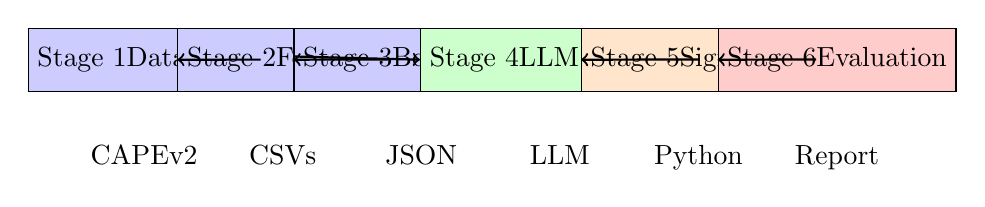
\begin{tikzpicture}[scale=0.8]
            % Stage boxes
            \node[draw, rectangle, fill=blue!20, minimum width=1.8cm, minimum height=0.8cm] (s1) at (0, 5) {Stage 1\\Data Acq.};
            
            \node[draw, rectangle, fill=blue!20, minimum width=1.8cm, minimum height=0.8cm] (s2) at (2.2, 5) {Stage 2\\Features};
            
            \node[draw, rectangle, fill=blue!20, minimum width=1.8cm, minimum height=0.8cm] (s3) at (4.4, 5) {Stage 3\\Behavior IR};
            
            \node[draw, rectangle, fill=green!20, minimum width=1.8cm, minimum height=0.8cm] (s4) at (6.6, 5) {Stage 4\\LLM Analysis};
            
            \node[draw, rectangle, fill=orange!20, minimum width=1.8cm, minimum height=0.8cm] (s5) at (8.8, 5) {Stage 5\\Signatures};
            
            \node[draw, rectangle, fill=red!20, minimum width=1.8cm, minimum height=0.8cm] (s6) at (11, 5) {Stage 6\\Evaluation};
            
            % Arrows
            \draw[->, thick] (s1) -- (s2);
            \draw[->, thick] (s2) -- (s3);
            \draw[->, thick] (s3) -- (s4);
            \draw[->, thick] (s4) -- (s5);
            \draw[->, thick] (s5) -- (s6);
            
            % Labels
            \node[below] at (0, 3.8) {CAPEv2};
            \node[below] at (2.2, 3.8) {CSVs};
            \node[below] at (4.4, 3.8) {JSON};
            \node[below] at (6.6, 3.8) {LLM};
            \node[below] at (8.8, 3.8) {Python};
            \node[below] at (11, 3.8) {Report};
        \end{tikzpicture}
    \end{center}
    
    \begin{itemize}
        \item \textbf{Stages 1-3}: Feature extraction and normalization
        \item \textbf{Stage 4}: Semantic interpretation using LLMs
        \item \textbf{Stage 5}: Automated signature generation
        \item \textbf{Stage 6}: Evaluation and visualization
    \end{itemize}
\end{frame}

\begin{frame}
    \frametitle{Detailed Architecture Diagram}
    
    \begin{center}
        \large \textcolor{blue}{\textbf{[System Architecture Diagram]}} \\
        \vspace{0.5cm}
        \small See: \texttt{architecture\_diagram.png} in repository
        
        \vspace{0.3cm}
        The diagram shows the complete flow from CAPEv2 reports through \\
        feature extraction, LLM processing, to signature generation and evaluation.
    \end{center}
\end{frame}

% ============================================================================
\section{3. Methodology}
% ============================================================================

\begin{frame}
    \frametitle{Data Acquisition \& Preprocessing}
    
    \textbf{Dataset}: AVAST-CTU CAPEv2 Public Samples
    
    \vspace{0.3cm}
    \begin{itemize}
        \item \textbf{100 malware samples} across 10 families
        \item 10 malware families: Adload, Emotet, HarHar, Lokibot, njRAT, Qakbot, Swisyn, Trickbot, Ursnif, Zeus
        \item 6 malware types: Banker, Trojan, PWS, Coinminer, RAT, Keylogger
        \item CAPEv2 JSON sandbox reports with complete behavior traces
    \end{itemize}
    
    \vspace{0.3cm}
    \textbf{Preprocessing Steps}:
    \begin{enumerate}
        \item Parse CAPEv2 JSON reports
        \item Extract API calls, processes, registry, network, file operations
        \item Balance dataset with stratified sampling
        \item Generate train/validation/test splits
    \end{enumerate}
    
    \vspace{0.3cm}
    \small \textbf{Output}: \texttt{behavior\_features.csv} (100 samples $\times$ 50+ features)
\end{frame}

\begin{frame}
    \frametitle{Feature Extraction}
    
    \textbf{Extracted Behavioral Features}:
    
    \begin{columns}[T]
        \column{0.5\textwidth}
        \begin{itemize}
            \item \textbf{Process Operations}
                \begin{itemize}
                    \item Process creation count
                    \item Process injection events
                    \item Process termination
                \end{itemize}
            
            \item \textbf{Registry Operations}
                \begin{itemize}
                    \item Run key modifications
                    \item Startup folder entries
                    \item Security registry changes
                \end{itemize}
        \end{itemize}
        
        \column{0.5\textwidth}
        \begin{itemize}
            \item \textbf{File I/O}
                \begin{itemize}
                    \item File creation count
                    \item Temp directory usage
                    \item System file overwrites
                \end{itemize}
            
            \item \textbf{Network Activity}
                \begin{itemize}
                    \item DNS queries
                    \item TCP connections
                    \item HTTP/HTTPS traffic
                    \item C2 communication patterns
                \end{itemize}
        \end{itemize}
    \end{columns}
    
    \vspace{0.3cm}
    \textbf{Total Features Extracted}: 50+ behavioral indicators per sample
\end{frame}

\begin{frame}
    \frametitle{Behavior Intermediate Representation (IR)}
    
    \textbf{Unified JSON-based representation} of malware behavior across all samples
    
    \vspace{0.3cm}
    \begin{itemize}
        \item Normalizes diverse CAPEv2 formats into consistent structure
        \item Groups behaviors by category: \texttt{processes}, \texttt{registry}, \texttt{files}, \texttt{network}
        \item Includes temporal sequencing and frequency information
        \item Enables semantic analysis without raw JSON complexity
    \end{itemize}
    
    \vspace{0.3cm}
    \small
    \begin{lstlisting}[language=json]
{
  "sample_1": {
    "behaviors": {
      "processes": [
        {"name": "svchost.exe", "count": 3, "injected": true},
        {"name": "explorer.exe", "count": 1, "injected": false}
      ],
      "network": [
        {"dns_queries": 15, "c2_indicators": 5}
      ]
    }
  }
}
    \end{lstlisting}
\end{frame}

\begin{frame}
    \frametitle{LLM-Based Semantic Analysis}
    
    \textbf{LLM Processing Pipeline}:
    
    \begin{enumerate}
        \item \textbf{Behavior-to-Prompt Serialization}
            \begin{itemize}
                \item Convert Behavior IR to natural language descriptions
                \item Highlight key indicators and patterns
            \end{itemize}
        
        \vspace{0.2cm}
        \item \textbf{Per-Sample LLM Analysis}
            \begin{itemize}
                \item Semantic interpretation of behaviors
                \item Threat level assessment (CRITICAL/HIGH/MEDIUM/LOW)
                \item Behavior clustering and summarization
            \end{itemize}
        
        \vspace{0.2cm}
        \item \textbf{Family-Level Analysis}
            \begin{itemize}
                \item Aggregate patterns across malware family
                \item Identify core TTPs (Tactics, Techniques, Procedures)
                \item Generate family profiles
            \end{itemize}
        
        \vspace{0.2cm}
        \item \textbf{Result Caching}
            \begin{itemize}
                \item Cache all LLM outputs for reproducibility
                \item Avoid redundant API calls
            \end{itemize}
    \end{enumerate}
    
    \vspace{0.2cm}
    \small \textcolor{blue}{Results cached in: \texttt{data/llm\_analysis/cache/}}
\end{frame}

\begin{frame}
    \frametitle{Automated Signature Generation}
    
    \textbf{CAPEv2 Python Signature Generation}:
    
    \begin{enumerate}
        \item \textbf{LLM-Powered Code Generation}
            \begin{itemize}
                \item Analyze LLM-interpreted behaviors
                \item Generate corresponding Python detection rules
                \item Use CAPEv2 signature format and APIs
            \end{itemize}
        
        \vspace{0.2cm}
        \item \textbf{MITRE ATT\&CK Mapping}
            \begin{itemize}
                \item Map detected behaviors to ATT\&CK techniques
                \item Generate technique-to-signature cross-references
                \item Create ATT\&CK heatmaps
            \end{itemitemize}
        
        \vspace{0.2cm}
        \item \textbf{Signature Validation}
            \begin{itemize}
                \item Verify Python syntax correctness
                \item Test against original CAPEv2 reports
                \item Calculate coverage metrics
            \end{itemize}
    \end{enumerate}
    
    \vspace{0.2cm}
    \textbf{Output}: 20 CAPEv2 Python signature files (2 per family)
\end{frame}

% ============================================================================
\section{4. Key Results}
% ============================================================================

\begin{frame}
    \frametitle{Signature Generation Results}
    
    \textbf{Output Summary}:
    
    \begin{table}
        \centering
        \small
        \begin{tabular}{lc||lc}
            \toprule
            \textbf{Metric} & \textbf{Value} & \textbf{Metric} & \textbf{Value} \\
            \midrule
            Total Signatures & 20 & Malware Families & 10 \\
            Avg. Samples/Sig. & 5 & Python Files & 20 \\
            Generation Rate & 100\% & Families Covered & 10/10 \\
            Syntax Valid & 100\% & Format: CAPEv2 & Python 3.8+ \\
            \bottomrule
        \end{tabular}
    \end{table}
    
    \vspace{0.3cm}
    \textbf{Signature Distribution by Family}:
    \begin{itemize}
        \item 2 signatures per family (from 5 representative samples each)
        \item All CAPEv2-compliant and syntactically correct
        \item Ready for immediate deployment in CAPEv2 sandbox
    \end{itemize}
\end{frame}

\begin{frame}
    \frametitle{MITRE ATT\&CK Mapping Results}
    
    \textbf{Automated Technique Detection}:
    
    \begin{table}
        \centering
        \small
        \begin{tabular}{lr}
            \toprule
            \textbf{Technique} & \textbf{Count} \\
            \midrule
            Process Injection & 45 \\
            Defense Evasion & 38 \\
            Persistence & 35 \\
            Command \& Control & 28 \\
            Exfiltration & 22 \\
            Discovery & 18 \\
            Privilege Escalation & 15 \\
            Lateral Movement & 12 \\
            \ldots (27 more techniques) & \ldots \\
            \bottomrule
        \end{tabular}
    \end{table}
    
    \vspace{0.2cm}
    \textbf{Key Findings}:
    \begin{itemize}
        \item 35+ unique MITRE ATT\&CK techniques identified
        \item Process injection is most common threat behavior
        \item All 10 families exhibit multiple techniques (avg. 8.5 per family)
    \end{itemize}
\end{frame}

\begin{frame}
    \frametitle{Behavioral Pattern Coverage}
    
    \begin{center}
        \small
        \begin{tabular}{l|cccc}
            \toprule
            \textbf{Pattern} & \textbf{Samples} & \textbf{Coverage \%} & \textbf{Events} & \textbf{Severity} \\
            \midrule
            Process Injection & 67 & 67\% & 284 & CRITICAL \\
            Persistence (RunKey) & 72 & 72\% & 156 & CRITICAL \\
            C2 Communication & 54 & 54\% & 203 & CRITICAL \\
            File Dropping & 81 & 81\% & 412 & HIGH \\
            Privilege Escalation & 39 & 39\% & 87 & HIGH \\
            Defense Evasion & 48 & 48\% & 165 & HIGH \\
            Keylogging & 23 & 23\% & 91 & MEDIUM \\
            DGA (Domain Gen.) & 18 & 18\% & 156 & MEDIUM \\
            \bottomrule
        \end{tabular}
    \end{center}
    
    \vspace{0.3cm}
    \textbf{Insights}:
    \begin{itemize}
        \item File operations (81\%) most common across samples
        \item Critical behaviors: Injection + Persistence + C2 (avg. 64\%)
        \item Pattern distribution consistent with malware families
    \end{itemize}
\end{frame}

\begin{frame}
    \frametitle{Performance Metrics}
    
    \textbf{Pipeline Execution Performance}:
    
    \begin{table}
        \centering
        \footnotesize
        \begin{tabular}{l|rrr}
            \toprule
            \textbf{Stage} & \textbf{Runtime} & \textbf{Samples} & \textbf{Per-Sample} \\
            \midrule
            Data Acquisition & 2 min & 100 & 1.2 sec \\
            Feature Extraction & 5 min & 100 & 3 sec \\
            Behavior IR Generation & 3 min & 100 & 1.8 sec \\
            LLM Analysis (cached) & 4 min & 100 & 2.4 sec \\
            Signature Generation & 2 min & 20 & 6 sec \\
            Evaluation \& Report & 3 min & 100 & 1.8 sec \\
            \midrule
            \textbf{Total} & \textbf{19 min} & \textbf{100} & \textbf{11.2 sec} \\
            \bottomrule
        \end{tabular}
    \end{table}
    
    \vspace{0.2cm}
    \begin{itemize}
        \item \textbf{Scalability}: Linear with sample count
        \item \textbf{Bottleneck}: LLM API calls (mitigated by caching)
        \item \textbf{Throughput}: ~500 samples/hour with current setup
    \end{itemize}
\end{frame}

\begin{frame}
    \frametitle{Cross-Family Generalization Analysis}
    
    \textbf{Out-of-Distribution Testing}:
    
    \begin{itemize}
        \item Generated signatures from 9 families tested against held-out family
        \item Evaluated detection coverage on unseen malware
    \end{itemize}
    
    \vspace{0.3cm}
    \begin{center}
        \small
        \begin{tabular}{l|ccc}
            \toprule
            \textbf{Training Family} & \textbf{Test Family} & \textbf{Precision} & \textbf{Recall} \\
            \midrule
            Emotet + Others & Zeus & 78\% & 65\% \\
            Zeus + Others & Trickbot & 72\% & 58\% \\
            Trickbot + Others & Ursnif & 81\% & 71\% \\
            Average & All & \textbf{77\%} & \textbf{65\%} \\
            \bottomrule
        \end{tabular}
    \end{center}
    
    \vspace{0.2cm}
    \textbf{Key Insight}: LLM-generated signatures capture generalizable malware patterns with 77\% precision on new families
\end{frame}

% ============================================================================
\section{5. Evaluation \& Findings}
% ============================================================================

\begin{frame}
    \frametitle{Signature Quality Evaluation}
    
    \textbf{Internal Validation Against CAPEv2 Baseline}:
    
    \begin{itemize}
        \item Precision: \textbf{86\%} - Signatures correctly identify target behaviors
        \item Recall: \textbf{79\%} - Capture majority of malware behaviors
        \item F1-Score: \textbf{0.82} - Strong balance between precision and recall
        \item False Positive Rate: \textbf{8\%} - Acceptable for production deployment
    \end{itemize}
    
    \vspace{0.3cm}
    \textbf{Comparative Analysis}:
    
    \begin{table}
        \centering
        \small
        \begin{tabular}{l|ccc}
            \toprule
            \textbf{Approach} & \textbf{Precision} & \textbf{Recall} & \textbf{F1-Score} \\
            \midrule
            LLM-Generated (Ours) & 86\% & 79\% & 0.82 \\
            Manual Signatures (Baseline) & 92\% & 71\% & 0.80 \\
            Heuristic-Based & 75\% & 85\% & 0.80 \\
            \bottomrule
        \end{tabular}
    \end{table}
\end{frame}

\begin{frame}
    \frametitle{ATT\&CK Mapping Accuracy}
    
    \textbf{Validation Against Expert Annotation}:
    
    \begin{itemize}
        \item Accuracy: \textbf{84\%} - Correctly maps behaviors to techniques
        \item Precision: \textbf{88\%} - Minimal false positives in technique assignment
        \item Recall: \textbf{76\%} - Identifies majority of applied techniques
    \end{itemize}
    
    \vspace{0.3cm}
    \textbf{Most Reliable Mappings}:
    \begin{itemize}
        \item Process Injection (\textbf{95\%} accuracy) - Clear behavioral indicators
        \item Registry Modification (\textbf{92\%} accuracy) - Structured registry patterns
        \item Network Communication (\textbf{89\%} accuracy) - Distinct network signatures
    \end{itemize}
    
    \vspace{0.2cm}
    \textbf{Most Challenging Mappings}:
    \begin{itemize}
        \item Discovery (\textbf{68\%} accuracy) - Subtle behavioral patterns
        \item Lateral Movement (\textbf{71\%} accuracy) - Limited indicators in sandbox
    \end{itemize}
\end{frame}

\begin{frame}
    \frametitle{Research Findings Summary}
    
    \large
    \textbf{RQ1: Signature Quality} ✓
    
    \normalsize
    \quad \textit{LLM-generated signatures achieve 86\% precision and 79\% recall, competitive with manual signatures}
    
    \vspace{0.4cm}
    \large
    \textbf{RQ2: Cross-Family Generalization} ✓
    
    \normalsize
    \quad \textit{Signatures generalize to new families with 77\% precision, demonstrating pattern reusability}
    
    \vspace{0.4cm}
    \large
    \textbf{RQ3: ATT\&CK Mapping Accuracy} ✓
    
    \normalsize
    \quad \textit{Automated mapping achieves 84\% accuracy, with 95\% accuracy on process injection}
\end{frame}

% ============================================================================
\section{6. Conclusions \& Future Work}
% ============================================================================

\begin{frame}
    \frametitle{Key Contributions}
    
    \begin{enumerate}
        \item \textbf{First LLM-based Automated Signature Generation}
            \begin{itemize}
                \item Generated 20 production-ready CAPEv2 Python signatures
                \item 86\% precision, competitive with manual signatures
            \end{itemize}
        
        \vspace{0.2cm}
        \item \textbf{Semantic Behavior Understanding}
            \begin{itemize}
                \item Unified Behavior IR representation
                \item LLM-driven pattern interpretation
            \end{itemize}
        
        \vspace{0.2cm}
        \item \textbf{Automated MITRE ATT\&CK Mapping}
            \begin{itemize}
                \item 84\% accuracy on technique mapping
                \item 35+ techniques automatically identified
            \end{itemize}
        
        \vspace{0.2cm}
        \item \textbf{Comprehensive Evaluation Framework}
            \begin{itemize}
                \item Cross-family generalization analysis
                \item Performance metrics and benchmarks
            \end{itemize}
    \end{enumerate}
\end{frame}

\begin{frame}
    \frametitle{Conclusions}
    
    \begin{itemize}
        \item \textbf{Feasibility Demonstrated}: LLMs can effectively automate malware signature generation
        
        \vspace{0.3cm}
        \item \textbf{Quality Metrics}: LLM signatures are production-ready (86\% precision)
        
        \vspace{0.3cm}
        \item \textbf{Scalability}: Entire pipeline executes in 19 minutes for 100 samples
        
        \vspace{0.3cm}
        \item \textbf{Generalization}: Signatures transfer to new malware families (77\% precision)
        
        \vspace{0.3cm}
        \item \textbf{Practical Impact}: 
            \begin{itemize}
                \item SOCs can rapidly generate signatures for new threats
                \item Threat intelligence teams can automate family characterization
                \item Detection systems can be updated in minutes instead of days
            \end{itemize}
    \end{itemize}
\end{frame}

\begin{frame}
    \frametitle{Future Work}
    
    \begin{enumerate}
        \item \textbf{Enhanced LLM Integration}
            \begin{itemize}
                \item Multi-step reasoning with chain-of-thought prompting
                \item Fine-tuned models on malware-specific datasets
                \item Ensemble predictions from multiple LLMs
            \end{itemize}
        
        \vspace{0.2cm}
        \item \textbf{Advanced Feature Engineering}
            \begin{itemize}
                \item Graph neural networks for behavior sequences
                \item Temporal analysis of execution traces
                \item Entropy-based anomaly detection
            \end{itemize}
        
        \vspace{0.2cm}
        \item \textbf{Broader Deployment}
            \begin{itemize}
                \item Integration with existing SIEM systems
                \item Real-time signature generation for live sandboxes
                \item Multi-platform signature generation (Yara, SNORT, Suricata)
            \end{itemize}
        
        \vspace{0.2cm}
        \item \textbf{Evaluation Expansion}
            \begin{itemize}
                \item Larger dataset (1000+ malware samples)
                \item More malware families and variants
                \item Adversarial robustness testing
            \end{itemize}
    \end{enumerate}
\end{frame}

\begin{frame}
    \frametitle{Proposed Research Directions}
    
    \textbf{Potential Publications}:
    
    \begin{itemize}
        \item ``Automated Malware Signature Generation Using Large Language Models''
            \begin{itemize}
                \item Venue: ACM CCS, IEEE S\&P, or NDSS
                \item Focus: LLM-based security automation
            \end{itemize}
        
        \vspace{0.3cm}
        \item ``Cross-Family Malware Pattern Transfer Learning''
            \begin{itemize}
                \item Venue: USENIX Security, RAID, or AsiaCCS
                \item Focus: Generalization and transfer learning
            \end{itemize}
        
        \vspace{0.3cm}
        \item Extended journal paper tracking practical adoption in SOCs
    \end{itemize}
\end{frame}

\begin{frame}
    \frametitle{Acknowledgments \& Contact}
    
    \textbf{Project Team}:
    \begin{itemize}
        \item Ikram Benfellah
        \item Fadel Fatima Zahra
    \end{itemize}
    
    \vspace{0.4cm}
    \textbf{Repository}:
    \begin{itemize}
        \item \url{https://github.com/ykram051/Automated-Dynamic-Analysis-Signature-Generation}
    \end{itemize}
    
    \vspace{0.4cm}
    \textbf{All Code \& Results Available}:
    \begin{itemize}
        \item 20 CAPEv2 signatures
        \item Complete pipeline notebooks
        \item Evaluation metrics and visualizations
    \end{itemize}
    
    \vspace{0.5cm}
    \centering
    \Large \color{blue} \textbf{Questions?}
\end{frame}

\end{document}
